\section{Experiments}
\textbf{Protocol.} Training uses 35,927 Grasp-Anything++ scenes (183,559 prompt--grasp pairs) and validation 734 scenes. Testing follows the official LGD seen/unseen split, restricted to annotated pairs: 1,376 seen and 601 unseen from 727 of 803 object keys. Test scenes, and training pairs whose object name is an unseen test name, are excluded from training; a word search finds unseen names in 5,332 training prompts, all as parts of other objects (e.g. a spoon's ``bowl''), and 40 of the 41 seen names occur in training. A top-1 grasp is correct if its IoU exceeds 0.25 and its angle error is below $30^\circ$ for some ground-truth grasp of the prompted part; $H$ is the harmonic mean of seen and unseen success. All runs use AdamW (lr $10^{-3}$, weight decay $10^{-4}$, 500 warm-up steps, cosine), batch 32 and 6 epochs on one T4; checkpoints are selected on 1,000 validation pairs.

\begin{figure}[t]
\centering
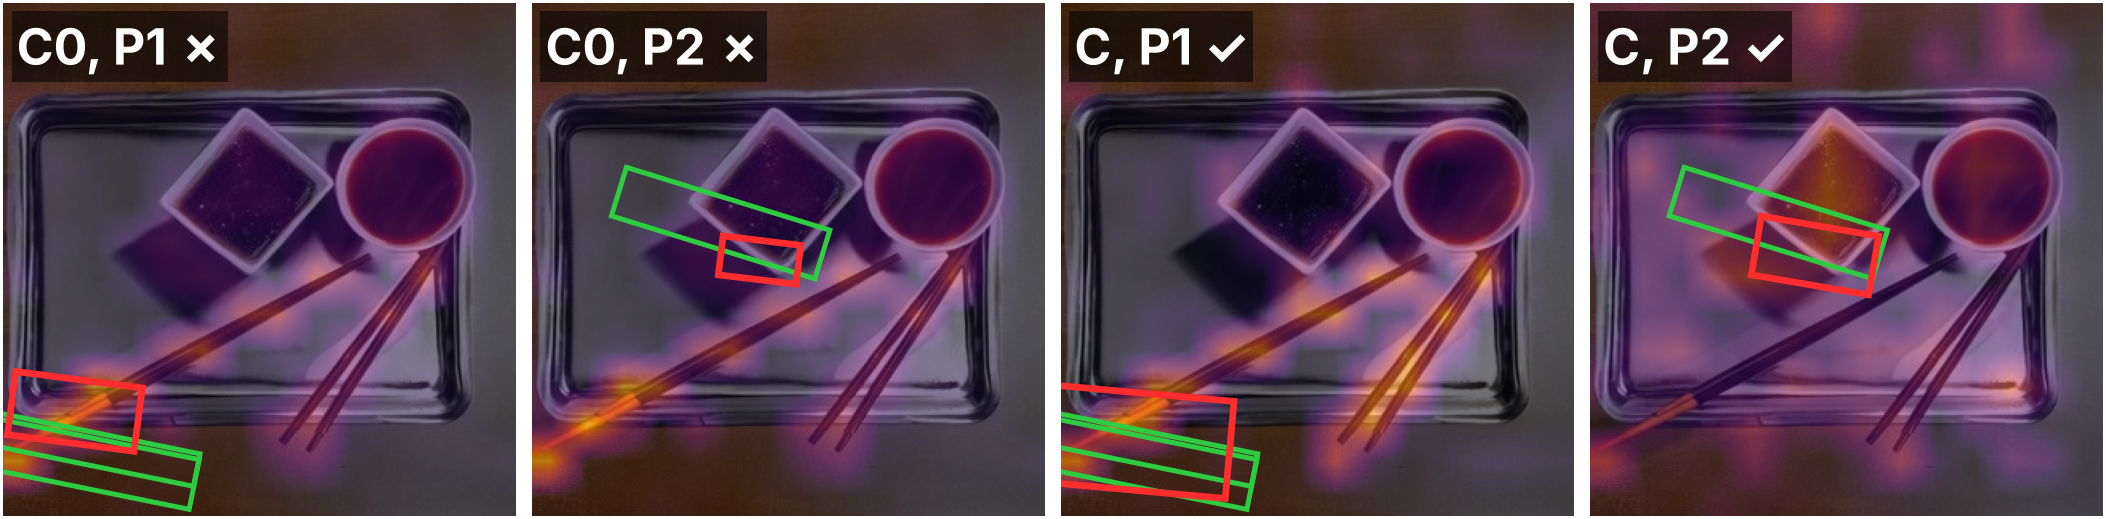
\includegraphics[width=\linewidth]{fig/gate.png}
\caption{\textbf{Gate maps} (heat), top-1 grasps (red), GT (green); unseen image, seed 0. P1: ``Hold chopsticks at its pair of sticks''; P2: ``Take hold of bottle on its container''. The C0 gate ignores the prompt; the C gate follows it. Selected as the largest C-gate change where only C is correct for both prompts.}
\label{fig:qual}
\end{figure}

\begin{table}[t]
\centering
\small
\setlength{\tabcolsep}{1.6pt}
\begin{tabular}{@{}llcccc@{}}
\toprule
 & Model & Seen & Unseen & $H$ & ms \\
\midrule
A & GR-ConvNet (RGB only) & 27.3 & 27.8 & 27.5 & 4.7 \\
B & + FiLM$(t)$ & 54.8$_{\pm2.7}$ & 40.7$_{\pm0.6}$ & 46.7$_{\pm1.4}$ & 14.1 \\
C0 & B + text-free gate & 63.3$_{\pm0.5}$ & 46.0$_{\pm1.9}$ & 53.3$_{\pm1.1}$ & 19.6 \\
\rowcolor{cvprblue!10}
C & B + language gate & \textbf{68.6}$_{\pm0.4}$ & \textbf{57.7}$_{\pm1.8}$ & \textbf{62.7}$_{\pm1.3}$ & 19.7 \\
D & C + gate supervision & 70.8 & 57.7 & 63.6 & 21.5 \\
\bottomrule
\end{tabular}
\caption{\textbf{Success rate (\%) on the annotated test split.} B, C0, C: two-seed mean${\pm}$half-range. ms: batch-1 T4 latency incl.\ CLIP.}
\label{tab:main}
\end{table}

\textbf{Results.} FiLM (B) raises $H$ by 19.2 points, CLIP features behind the text-free gate (C0) add 6.6, and letting the gate read the prompt (C) adds 9.4. Seed for seed, C exceeds C0 by 11.6/11.8 unseen and 6.3/4.4 seen points; paired McNemar tests give $p<10^{-3}$ in all four comparisons, and scene-resampled 95\% bootstrap intervals exclude zero. The unseen gain of C0 over B varies between seeds ($+7.8$, $p<10^{-3}$; $+2.8$, $p=0.21$), whereas the C0$\to$C gain does not. C is correct for two prompts on different objects in 54 of the 118 multi-object test scenes, C0 in 40 (seed 0, \cref{fig:qual}). Prompt-dependent gating thus gives 69\% of the B$\to$C gain on unseen objects, 59\% in $H$ and 38\% on seen ones. D does not differ significantly from C (seed 0; $p\geq0.06$), so C is kept.

\textbf{Cost and limitations.} C adds 0.33M trained parameters to B and a frozen 149M-parameter CLIP (13.0\,ms per frame with a cached prompt) and trains on 3.6\% of the images. A exceeds the 18 unseen reported for GR-ConvNet with CLIP in~\cite{vuong2024language}, so LGD's 48/42 are not compared.
